\documentclass[jou,draftfirst,11pt]{apa6}
\usepackage[english]{babel}
\usepackage[utf8]{inputenc}
\usepackage{booktabs}
\usepackage{tabularx}
\usepackage{csquotes}
\usepackage{caption}
\usepackage{rotating}

\usepackage{tikz}
\usetikzlibrary{positioning,shapes,arrows,calc}
\usetikzlibrary{shapes.geometric,shadows,shapes.misc}
\tikzstyle{every text node part}=[font=\fontsize{10}{11}\selectfont]

\usepackage[
  style=authoryear,
  dashed=false,
  bibstyle=authortitle,
  backend=biber]{biblatex}
\renewcommand\nameyeardelim{, }
\bibliography{arousal.bib}

\defbibheading{bib}[References]{%
                \newpage\section{#1}%
                \markboth{#1}{#1}}


\AtBeginBibliography{%
  \renewcommand*{\finalnamedelim}{%
    \ifnumgreater{\value{liststop}}{2}{\finalandcomma}{}%
    \addspace\&\space}%
}


\let\origparencite\parencite
\renewrobustcmd{\parencite}{%
  \AtNextCite{%
  \renewcommand*{\finalnamedelim}{%
    \ifnumgreater{\value{liststop}}{2}{\finalandcomma}{}%
    \addspace\&\space}%
  }%
  \origparencite%
}


\newcommand{\cellcontent}[1]{\begin{tabular}[t]{@{}l@{}}#1\end{tabular}}



\title{Arousal and Post Decision Processes: Effects of Experimentally
  Manipulated Arousal on Differentiation and Consolidation Processes.}

\shorttitle{Arousal and Post Decision Processes}

\author{Johanna V. Almtoft and Mats O.L. Nyberg}
\affiliation{Departement of Psychology, University of Lund}

%\authornote{Authornote}
\note{Bachelor thesis, PSY 141\\
  Supervisor: Ilkka Salo\\
  Examinator: Sven-Birger Hansson}


\abstract{This study investigates experimentally manipulated arousal influence
on post decision consolidation processes within the theoretical
framework of the differentiation and consolidation theory of human
decision making \parencite{svensson92b}.  Fifty-six university students
participated in the experiment.  Instructional manipulation of
participants' level of arousal was used. A multi-attribute decision
task concerning a choice between two apartments was used.  One week
later the participants  had to recall the task.  Heart rates were
measured using a heart rate meter, and current mood assessed using a
questionnaire \parencite{LewinsohnMano93}.  Results of  the arousal
manipulation were not found, nor any consolidation effect (F-test,
$\alpha$=.05).  No importance reversals of alternative attributes occurred.
Interaction effects between commitment, activation level, level of
arousal, conflict and ability to recall variables were not found
(Tukey's HSD, $\alpha$=.05).  The conclusion was that predictions failed due
to too weak a manipulation of arousal.  Implications for future
research were discussed.}

\keywords{Differentiation and Consolidation Theory, Arousal, Mood,
  Heart Rate, Decision Making}

\begin{document}
\maketitle


This study investigates the effects of arousal on decision making
processes.  Decision making is an activity people engage in on an
everyday basis.  Decisions differ in  their impact on the decision
maker's life, and the stakes involved.  How we reach our decisions and
how we view them in hindsight are issues that concern researchers
within decision making theory, a field of cognitive and social
psychology.


\subsection{Decision making theory}

Early, primarily structural decision making theories, focused
primarily on the results of the decisions.  Major theories among these
are expected utility theory (EU),  subjective expected utility theory
(SEU), and multi attribute utility theory (MAUT) (cf., \cite{baron94}).
EU is a normative theory in so much as it provides researchers with
means to evaluate decisions made under ideal circumstances.  According
to EU, the decision maker carefully weights the utility of the outcome
of each alternative against the probability that the outcome will
occur when choosing the alternative.  SEU is similar to EU except that
the decision maker weights the utility of the outcome against the
subjective probability of the outcome when comparing alternatives.  In
MAUT, the utility of an alternative is calculated by breaking each
consequence of the alternative into attributes.  The utility of each
attribute of each option is measured and added across the attributes
\parencite{baron94}.

Subsequent process related decision making research focus on decision
making over time and the underlying processes. Lewin (\cite{lewin51}; as
cited in \cite{festinger64}), studied both pre- and post decisional
processes and found differences between them.  According to him, the
decision maker investigates and compares the different alternatives in
an objective manner prior to the decision.  After the decision is
made, the decision maker shows tendencies to stick to the values and
opinions about the alternatives held in the moment the decision was
made, even in the light of contradictory information (\cite{lewin51}; as
cited in \cite{festinger64}).


\subsection{Conflict and dissonance}

In cognitive dissonance theory \parencite{festinger64}, the differences
between pre and post processes in decision making are considered and
incorporated.  In making a decision, Festinger claims, the decision
maker collects equal amounts of information and compares their good,
as well as their bad aspects.  The attributes are compared according
to a preference list and the alternatives are systematically
re-evaluated in order to find a difference between the attractiveness
of the best alternative and the others large enough to choose it.

According to Festinger, a conflict in the pre decision phase is
followed by dissonance in the post decision phase.  A conflict occurs
when the attractiveness of the choice-alternatives at hand are so
close that no choice is obvious.  Having to choose either of the
alternatives, then causes the decision maker to feel a frustration, as
a sign of a conflict.  Festinger also found that participants
considered their decision to a higher extent when the difference
between the alternatives' attractiveness was close, and when the
decision makers were committed to the issue of the decision.
Immediately after the decision is made the decision maker starts
question the choice, looking for facts that speak against the chosen
alternative.  If the decision maker under this phase finds
inconsistencies between the choice and personal values, dissonance
occurs.  The greater the conflict before the decision is made, the
greater the dissonance afterwards \parencite{festinger64}.  As this
dissonance is perceived as threatening to the decision maker, a
dissonance reduction process starts.  This consists of a selective
continued consideration of the alternatives' attributes, e.g. by
looking for facts related to the decision that supports the chosen
alternative.  The dissonance reduction continues until the decision
maker feels content in standing by the decision
\parencite{festinger64}.

These pre and post decision processes mentioned by Festinger
\parencite{festinger64} are also brought up in Conflict, Choice and
Commitment theory \parencite{JanisMann77}.  In their conflict model of
decision making they regard the decision maker as unwilling to act.
The decision maker acts only when challenged by some warning that the
present situation is threatened, and then starts to consider the
choice-alternatives.  Janis and Mann describe the decision making
process by means of a flow chart.  The decision making process
consists of antecedent conditions, mediating processes and the
consequences of the decision.  In the model the present decision
situation is preceded by a number of antecedent conditions, that gives
information to direct the decision maker in the choice of future
course of action (i.e.  to make a choice between alternatives).  After
the decision is made Janis and Mann predicts post decision processes.
The decision maker often strengthen, ``bolster'', the decision after it
is made.  Bolstering increases with the degree of conflict in the
decision.  The decision maker often alters the subjective appraisal of
the alternatives in favour of the chosen one.  In doing this, the
decision maker often follow one out of a set of bolstering strategies.
Janis and Mann discusses six such strategies.  The decision maker can,
for instance, choose to exaggerate positive consequences or downgrade
negative consequences of the decision.  The decision maker may also
deny threatening emotions (e.g. to see the chosen course of action as
a challenge), exaggerate the remoteness of the action commitment,
minimising social surveillance or the decision maker may minimise the
feeling of personal responsibility.  The choice of strategy depends on
personal factors, but also on the situation as well as the kind of
decision in question.

\subsection{The differentiation and consolidation theory
  (diff. con. theory)}

The diff. con. theory \parencite{svensson92b, Svensson95} takes the
suggestions made by Festinger \parencite{festinger64} as well as Janis
and Mann \parencite{JanisMann77} into further consideration.  According to the
diff. con. theory, the decision maker, when put in front of a number
of alternative courses of action, starts to scrutinise the
alternatives in order to distinguish them from each other, this is
called the differentiation process.  The differentiation process works
gradually, and the aim here is to get one of the alternatives, not
only the best but so much better that the choice will stand solid in
the future. The chosen alternative have to be superior even in the
occurrence of new information that might decrease the difference in
attractiveness, obtained in the differentiation process,  between the
chosen and the competing alternatives.  Such new information can be
either external (e.g., poor outcome) or internal (e.g., change in own
values) and constitutes a threat to the superiority of the chosen
alternative \parencite{svensson92a}.  The corresponding post decision
process in support of the chosen alternative is called consolidation.


\subsection{Differentiation}

When confronted with a decision problem, the decision maker starts
identifying the alternatives and goals by means of available
information.  In order to minimise the strain on the decision maker,
perceptual or cognitive markers, presumably, shows where to start the
analysis.  Such a marker might, for instance, tell the decision maker
to start by looking at the price of an alternative.

Three different types of differentiation processes are identified:
holistic, process related and structural.  Svensson
(\citeyear{svensson92b}) connects these types of differentiation to
four levels of decision making based on the representation of
attractiveness needed at each level.  People tend to use holistic
differentiation in quick decisions at level one and two.   Decisions
belonging to level one are the simplest.  These are made automatically
and the alternatives do not need any direct representation of
attractiveness as the decisions are made on a basis of similarity with
preceding decisions.  Instead the decision maker uses other cognitive
processes (for instance matching).  Decisions at this level may once
have belonged to higher levels but through application and experience
they have been reduced and are now made automatically.  Such a
decision can, for instance, be to always buy a certain brand of
breakfast cereal without considering other alternatives.  A reference
decision alternative is often chosen through a quick, level one
decision to be used as an anchor, a point of reference to which other
alternatives are compared during the subsequent differentiation.
Decisions made at level two refers to the alternatives attractiveness
of one or more attributes.  The decisions are made according to some
stereotypic rule of thumb, for instance ``big is beautiful''.  Another
way to make a decision at this level is to consider the attractiveness
in a holistic perspective in the sense that the decision is made,
based on emotions or intuition.  Such decisions can, for instance be
to help out in a situation according to the notion that ``helping is
good''.  The decision maker can also appraise the alternatives'
attractiveness in a holistic way, e.g. on emotional or intuitive
basis.  It is often enough with this kind of differentiation in order
to make a decision but the holistic differentiation may also be a part
of a more complex differentiation process \parencite{svensson92b,
  Svensson96}.

The process of differentiation may follow one or more decision
rule(s).  These rules guides the decision maker in his reasoning to
obtain the best choice.  The decision rules, however, do not suggest a
good differentiation level, the difference in attractiveness to aim
for.  The choice of rules depends on both personal and situational
factors \parencite{svensson92b}.  Such kind of decision rules, are the
conjunctive and the compensatory rules \parencite{Svensson96}.  When
applying conjunctive decision rules to a decision, criterion values
for each attribute are set up.  Each alternative is then measured
against these criterion values attributewise, and are rejected if they
fall below the criterion.  This proceeds, if possible, until one
alternative stands as a sole winner.  Compensatory rules, on the other
hand, assume that the alternatives have attractiveness values that are
comparable across different attributes.  Compensatory rules may then
prescribe the decision maker to look for the attribute with the
greatest difference in attractiveness and then choose the alternative
which is more attractive on this attribute or the decision maker could
choose the alternative with the largest number of favourable
attributes.

In the process oriented differentiation, the alternatives are
distinguished through decision rule differentiation or criterion
differentiation.  In decision rule differentiation it is common to
start the differentiating process using rules like the conjunctive
rule to eliminate some of the possible initial alternatives.  In the
next phase of the decision process, rules using trade-offs between
choice-attributes (e.g. compensatory rules) are applied.  In criterion
differentiation criterion values on different attributes are set up by
the decision maker according to subjective values.  The different
kinds of decision rules used in the process related differentiation
all need these criteria.  Alternatives that does not meet this
criterion can be sorted out.  If there are too many alternatives
remaining either criterion or rules can be changed \parencite{Svensson96}.

 The main focus of the diff. con. theory has been on the structural
 differentiation process and on decisions belonging to level three .
 Decisions at level three are not made automatically. The
 alternative's attractiveness are considered and assessed during
 differentiation since the choice here often involves a conflict.
 According to diff. con. theory a conflict occurs when the chosen
 alternative is inferior to competing alternatives regarding the value
 of an important attribute.  The decision maker sometimes changes
 their appraisal of the decision, following a number of decision
 rules, in order to strengthen their decision \parencite{Svensson95}.
 This restructuring may involve attractiveness, importance of
 alternatives' attributes and facts as well as the decision problem.
 A choice at this level might, for instance, be a choice between two
 cars.  To decide on a car, attributes (aspects of the cars) are
 compared according to the decision makers' subjective estimate of
 their importance (e.g. colour, security and price) before the
 decision is made.

 Restructuring with respect to attractiveness often takes the form of
 upgrading the chosen alternative's attractiveness and / or downgrade
 the rejected alternatives' attractiveness.  Restructuring with
 respect to attribute importance consists of a change in rank order
 between the attributes constituting the alternatives.  Factual
 restructuring occurs, for instance, when forced to reject a preferred
 car and buy a cheaper, less preferred car.  Factual restructuring can
 then have the effect of making the buyer remember the price of the
 more expensive car as even higher than it really was.  Restructuring
 of decision problems consists for instance of looking for new kinds
 of solutions to the problem.  When the alternatives are unknown, in
 full or to some extent, the decision maker have to find out the
 alternatives.  For instance, finding out the best way to invest a sum
 of money may involve searching for and appraise different means and
 opportunities to place the money, perhaps new to the decision maker.
 Such a decision belongs to level four.  The situations leading
 towards the decisions of level four are often novel to the decision
 maker and because of this the decisions may involve aspects of
 problem solving \parencite{svensson92b}.


\subsection{Consolidation}

In having to choose one alternative over the others, includes a threat
in the sense that it involves loosing the good aspects of the rejected
alternatives as well as the fact that the decision maker gets stuck
with negative aspects of the chosen alternative.  A way to reduce this
threat is, as the diff. con. theory predicts, to continue the process
of differentiation after the decision is made.  This post decision
differentiation process is called the consolidation process.  The same
processes as in the differentiation are used and the restructuring now
occur in order to strengthen the decision.  The level of restructuring
depends on the size of the difference between the chosen alternative
and the rejected.  If the difference between the alternatives with
respect to the most important attribute already is well established
(so that the choice is undoubted), the need to consolidate is lower
and this allow for attention to the other attributes of the
alternative (the second, the third and so on...).  Consolidation
continues as long as the decision maker feels doubts regarding the
choice.

Svensson and Benthorn performed studies of importance and facts
restructuring on mainly fictions decision making tasks without real
outcome \parencite{svensson92a}.  They focused on the post
decision processes that occur in order to consolidate a previously
made choice.  In one study \parencite{svensson92a} no
consolidation effect was observed five minutes after the decision was
made, but after a week had passed, consolidation did occur regarding
attractiveness favouring the chosen alternative,  in terms of
upgrading the aspect values from the first occasion to the second.
This effect concerned only the two most attractive attributes.  This
effect was the opposite, regarding the two least important attributes
where the difference had decreased.

Svensson and Malmsten (\citeyear{SvenssonMalmsten95}) investigated the
effects of differentiation and consolidation processes regarding
decisions with real life alternatives and real outcomes
\parencite{SvenssonMalmsten95}. The participants had to choose between
either of two lotteries. The choice involved a conflict in terms of
attractiveness between the choice-alternatives and probability of the
desired outcome as the lottery with the finest price had the smallest
probability of wining and vice versa.  According to Svensson and
Malmsten, this conflict would increase the level of consolidation.
Results showed that the participants who received a positive outcome
from their choice, consolidated to such a degree that attributes that
were reported to decrease the chosen alternative's attractiveness
prior to the decision, afterwards were reported to be in favour of the
chosen alternative.  The participants whose choice gave a desired
outcome appreciated their chances to this outcome as being higher
after the decision than they did prior to the decision.  Participants
that did not get the desired outcome showed opposite, however not as
strong, results.

In another study, Svensson and Malmsten found a consolidation effect
after only ten to fifteen minutes after the decision was made, as
opposed to the study by Svensson and Benthorn (1992).  The cause of
this difference was assumed to be found in the fact that the later
study occurred under real life conditions as this increases the
commitment of the decision makers \parencite{SvenssonMalmsten95}.


\subsection{Mood and decision making}

In current research within the diff. con. theory framework there have
been a growing interest of the effects of process moderating factors
in the decision making processes.  This include stress, time pressure,
task involvement, mood and other factors that might affect the
decision maker \parencite{Svensson95}.  The focus of this study concerns the
influence of aspects of mood on post decision processes.


\subsection{Mood and emotion}

Mood is related to emotions and affect \parencite{FiskeTaylor91}. When a
person experience something, this might cause an affect. Affect stands
for a variety of preferences, evaluations, moods and emotions.
Preferences include mild subjective reactions that are essentially
either pleasant or unpleasant.  This have been studied within social
psychology, mainly regarding personal evaluations (i.e.  simple
positive and negative reactions to others).  Mood may be distinguished
from other affects in the fact that mood has a less specific target.
Being in a good mood does not necessarily have to have a specific
reason.  Moods affect a wide range of social cognitions and
behaviours. Like affect, moods are primarily considered as simply
positive or negative \parencite{FiskeTaylor91}.

The concept of emotion refers to a complex variety of affects, beyond
merely good and bad feelings, e.g. including anger, exuberance and
joy.  Emotions can cause intense feelings that may involve physical
manifestations, including increasing respiration and heart rate level
\parencite{FiskeTaylor91}.

Emotions and mood have also been distinguished in terms of external
versus internal concerns, object versus objectless focus and present
versus future orientation \parencite{FiskeTaylor91}.

Mood affects the whole human being.  It affects muscle tension,
neurological activity as well as the cardio-vascular system
\parencite{Izard77}.  There also exists a body of evidence on the fact
that our mood influence cognitions in the matter of self appraisal as
well as on our perception.  A persons mood in a specific situation
influence the way the person perceives the situation.  For instance, a
person in a positive mood is more likely to perceive the world through
``rose coloured glasses''.  Similarly may a negative mood ``pitch the
world black'' \parencite{Izard77}.

Several studies have showed that a high commitment and an interest in
a choice situation, makes the person willing to put in much cognitive
effort into the decision and consider facts related to the situation
\parencite{festinger64, Izard77, JanisMann77}.  Results have also
shown that subjects become more willing to make sacrifices in terms of
their own comfort.  The subjects who were given a good result on a
dummy test showed a greater willingness to put effort into charity
work than did subjects who were given a poor result \parencite{Weyant78}.
Shachter and Singer means that mood is a result of physiological
arousal, cognitive evaluation and an appraisal of the situation
causing the arousal \parencite{SchachterSinger62}.  Depending on the
evaluation of the situation where the arousal occurred, the person may
experience different kinds of mood.


\subsection{Arousal}

Researchers agree upon the notion of a correspondence between
psychological and physiological arousal \parencite{Atkinson93}.
Atkinson et al claims further that changes in
psychological arousal are closely related to and followed by changes
in physiological arousal.  Arousal resulting from activation of the
sympathetic division of the autonomic nervous system as it prepares
the body for emergency action can be observed through,
e.g. measurements of blood pressure and heart rate
\parencite{Atkinson93}.

Schedlowski and Tewes (\citeyear{SchedlowskiTewes92}) have studied the
relationship between self reports of experienced arousal and actual
arousal among novel and expert parachute jumpers, during jumps.
Results showed that the novel jumpers assessed their arousal during
the jump as being higher than the expert jumpers did.  Heart and
respiration rates showed similar levels of arousal between the two
groups.

Bagozzi (\citeyear{Bagozzi95}) have conducted studies in attitude
theory and  found 
that an increase of positive associations and cognitions concerning
actions as well as a decrease in negative associations and cognitions
follow an increase in arousal. This can be related to studies by
Elliot and Devine (\citeyear{ElliotDevine94}), who found that arousal
manipulation facilitates task performance on easy tasks, but decrease
task performance on hard tasks.

Results from studies on learning and arousal have shown a
correspondence between a state of high commitment and interest with a
high level of physiological arousal (\cite{Berlyne60} as cited in
\cite{Izard77}; \cite{Berlyne67}; as cited in \cite{Izard77}).

Results from other studies have shown on an opposite U-shaped
relationship between arousal and information processing capacity.  Up
to a certain point, an increase in arousal results in an increase in
commitment and interest.  Beyond this point, however, the arousal
results in tunnel vision, concentration difficulties or hypervigilance
(e.g. \cite{Easterbrook59}; \cite{JanisMann77}; \cite{LewinsohnMano93};
\cite{StoneKadous94}).



\subsection{Mood, arousal and decision making}

Research have been conducted on the influence of mood on cognitions in
general.  Some research have focused on the effect of mood in decision
making.  In studies of the effect of mood on decision making
processes, Lewinsohn and Mano refers to a multi dimensional mood state
model \parencite{LewinsohnMano93, Mano94} (see Figure
\ref{fig:circumflex}), This model
is a development of Russel's multi dimensional mood model
\parencite{Russel78}. In Mano's model mood is described on two main dimensions,
hedonic tone (pleasure-displeasure) and arousal (arousal-quietness).
Besides these main dimensions the model includes locus of causation,
control as well as the depth of experience they are assumed to explain
only a minor part of the variance.  In the model, Mano includes eight
discrete mood states \parencite{Mano94}.






\begin{figure}
  \begin{center}
    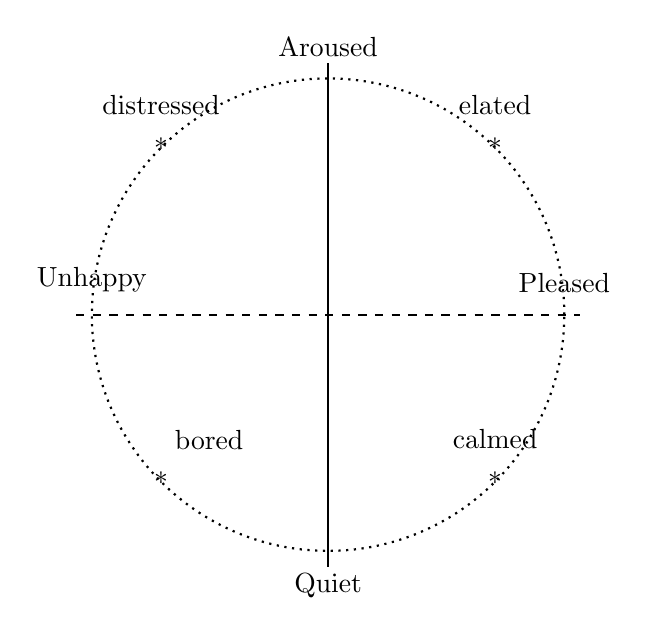
\begin{tikzpicture}[>=stealth',shorten >=0pt,node distance=1cm,
    every label/.style=label distance=10mm
]
      \node [label={90:Aroused}] (aroused) at (90:3) {};
      \node [label={90:Pleased}] (pleased) at (0:3) {};
      \node [label={90:Unhappy}] (unhappy) at (180:3) {};
      \node [label={270:Quiet}] (quiet) at (270:3) {};

      \node [label={90:elated}] (elated) at (45:3) {*};
      \node [label={90:distressed}] (distressed) at (135:3) {*};
      \node [label={80:bored}] (bored) at (225:3) {*};
      \node [label={90:calmed}] (calmed) at (315:3) {*};

      \draw [thick,dotted] (0,0) circle (3cm);

      \draw [thick,dashed] ($(unhappy)+(-0.2,0)$) -- ($(pleased)+(0.2,0)$);
      \draw [thick] ($(quiet)+(0,-0.2)$) -- ($(aroused)+(0,0.2)$);

    \end{tikzpicture}
  \end{center}
  
  \caption{The Affect Circumplex \parencite{LewinsohnMano93}.}
  \label{fig:circumflex}  
\end{figure}






In studying emotions, researchers distinguish experience of emotion
over time from current emotion \parencite{FiskeTaylor91}. For instance,
Watson and Tellegen (\cite{WatsonTellegen85}, as cited in \cite{FiskeTaylor91})
describes' the structure of affect by a two dimensional model, similar
to Manos' Affect Circumplex model parencite{Mano95}.

In a study, conducted by Lewinsohn and Mano
(\citeyear{LewinsohnMano93}), subjects were asked to give self reports
concerning their naturally occurring emotional state followed by a
multi-attribute decision making task. This study showed that subjects
in a pleasant mood put more cognitive effort into their decision than
did subjects in more aroused mood. Subjects in an aroused mood spent
less time elaborating the alternatives of the decision making task.
They also considered fewer attributes and made less comparisons
between the alternatives.

Psychologists have addressed the problems in inducing specific
discrete mood states \parencite{Izard77, Polivy81}.  Trying to induce
one specific mood often result in multiple dimensional states
\parencite{Polivy81}.

Studies have been performed on the influence of arousal on post
decision processes.  Benson III (\citeyear{Benson93}) have conducted
such studies on 
post decision processes and framing when the decision is made under a
time constraint.  He does, however, not distinguish arousal, induced
by a time constraint from general arousal \parencite{Benson93,
  Svensson96}.  Svensson and Edland (\citeyear{SvenssonEdland87})
assumes, however, that arousal induced by a time constraint and
general arousal may both result in a reduction in information
processing capacity and will therefore affect decision making
processes equally.

Salo (\citeyear{Salo96}) has brought decision and mood theory together
in a study concerning the influence of manipulated negative and
positive mood on post decision processes.  In order to induce
different moods, subjects were asked to recollect a personal memory of
a situation in which the specific mood had been particularly strong.
After this subjects were given a decision task.  One week later the
subjects had to recall the attractiveness of the attributes of the
alternatives  of the decision making task.  Consolidation in terms of
restructuring of attractiveness differences between the chosen and the
non-chosen alternative did not occur in any condition.  There were,
however, within subject changes in post decision attribute
attractiveness restructuring of  the most important attributes,
following positive and negative mood.  Subjects in both conditions
tended to upgrade both alternatives, although this effect was stronger
in the group of subjects in positive mood than in the group of
subjects in negative mood.

Salo also found that subjects changed their rank order of attribute
importance from the first occasion to the second one more frequently
in negative than in positive mood which was assumed to be an
indication of insufficient differentiation of the alternatives.  Salo
(\citeyear{Salo96}) suggests that future research should focus on how
the arousal component of mood may contribute to possible effects on
differentiation and consolidation processes.


\subsection{Research questions}

According to diff. con. the differentiation  in the pre decision
processes are followed by consolidation in the post decision phase
\parencite{Svensson95}.  Arousal affects cognition differently in  different
situations \parencite{FiskeTaylor91}.  This may lead to different degrees
of differentiation which in turn may be followed by different degrees
of consolidation.  Being in an aroused state when making a decision,
may increase the consolidation in the post decision process, due to a
decrease in information processing, depending of the level of arousal,
which, in turn, may lead to a lower differentiation level.  On the
other hand being aroused during a decision making task may lead to a
decrease in consolidation \parencite{Svensson95}. This is due to  the fact
that, up to a certain point, an increase in arousal creates an
increase in the decision makers information processing capacity
\parencite{Easterbrook59}. This may enable the decision maker to
differentiate the alternatives enough to feel content regarding the
choice and will therefore not need to consolidate \parencite{svensson92b}.

Following research questions are asked here:  Does an experimentally
manipulated arousal in the decision making moment affect the
differentiation process in such a way that this in turn gives rise to
a consolidation process that differs from one that arises from a
differentiation not affected by an manipulated arousal?  If so, in
which directions are the consolidation process affected? Is the level
of consolidation increased or decreased by the manipulation compared
to the consolidation in a situation without manipulated arousal?  Will
reversals or restructuring of the attribute rank order of importance
occur following manipulated arousal? In case of initial value
conflicts between the choice alternatives,  how are they solved by
decision makers with different levels of arousal?

\subsubsection{Hypothesis} Following hypothesis will be tested: Manipulated arousal
will lead decision makers to decrease their cognitive effort in
evaluating the alternatives of a decision making problem in the pre
decision phase to their decision.  This should affect the decision
makers' confidence in their choice which in turn influence the
consolidation process in the post decision phase compared to
participants without a manipulation of their level of arousal.


\section{Method}

\subsection{Participants}

Fifty-six university students (28 men, 28 women, mean age = 23.4
years) volunteered to participate in the experiment.  They were all
students at the Lund University, faculties of social sciences,
economics and law.  The distribution of participants between the two
conditions, experiment and control, can be seen in Table 1.




\begin{table}
  \centering
  \caption{Distribution of participants with respect to experimental
    condition and gender.}
  \label{table:participants}
  \begin{tabularx}{0.45\textwidth}{XXXXX}
    \toprule
    Condition & Men & Women & Totally & Mortality \\ 
    \midrule
    Experiment (Arousal) & 13 & 15 & 28 & 7 \\ &&&& (6.7\%) \\
    Control & 15 & 13 & 28 & 7 \\ &&&& (6.7\%) \\
    \bottomrule
  \end{tabularx}
\end{table}










The participants that showed up on both occasions had a chance to win
a IKEA gift voucher, worth 200 SEK.  Participants were guaranteed
confidentiality.


\subsection{Materials}

The following materials were used in the experiment: a heart rate
meter, a number of forms, a mood questionnaire and a demographic
report.  The demographic report was a 5 pages long report concerning
migration to and from the city of Lund.  The heart rate meter was a
Clas Ohlsson, PULSE BEEP, which use an active IR sensor to measure
pulse rate in the bloodflow on the left index finger.  The sound
system was disconnected to avoid interference.

\subsubsection{Forms} Six different forms were used.  One form (see Appendix A)
consisted of four VAS scales, (all VAS scales; visual analogue scales,
used in the experiment were one hundred millimetres) labelled with the
attribute names.  They were anchored from ``unimportant'' to ``important''
in the end points.

The decision task (see Appendix B) consisted of two equally attractive
apartments described with respect to the four attributes named above.
The attribute values of the both apartments were presented with eight
VAS-scales, anchored from ``good'' to ``bad'' in their end points.  Each
scale was labelled with an attribute name and a mark showing the value
of the attribute of the apartment.

A questionnaire (see Appendix C) contained questions about any
strategies used in the decision making task and regarding commitment
to as well as conflict in the decision.

Three forms were to be presented on a second occasion.  The first of
these (see Appendix D) resembled the decision making task, but the
marks on the VAS-scales were missing (see Appendix B),

A second form (see Appendix E) resembling the importance form
(Appendix A) was used to assess participant preferences with respect
to the four attributes.  This form also contained a VAS scale,
anchored from ``easy'' to ``hard'', used to assess participants difficulty
to remember the apartments aspect values.

A third form (see Appendix F) was a questionnaire about participant's
experiences from the different phases of the experiment, also
including two VAS scales (anchored from ``calm'' to ``active'' and from
``little'' to ``much'', respectively) where participants were asked for a
self report of ``how active they were during the decision task'' and the
extent to which this influenced the decision task.


\subsubsection{Mood questionnaire} 
A mood questionnaire (see Appendix G) was used
consisting of twenty-four items.  The items were grouped by the eight
octants in Mano's Affect Circumplex.  Each item consisted of mood
related adjective followed by a VAS-scale, anchored from ``not at all''
to ``a lot'' in the end points.  The mood questionnaire is a development
of Mano \parencite{LewinsohnMano93} to fit Swedish circumstances
(language) \parencite{Salo96}.  The following alphas (Cronbach) for
covariance among the three items per octants have been obtained:
arousal (0.70), elation (0.78), pleasantness (0.81), calmness (0.46),
quietness (0.49), boredom (0.85), unpleasentness(0.92), distress
(0.69).


\subsection{Procedure}

The experiment was conducted at the Department of Psychology, Lund
University, Sweden.  Participants were selected through a simple
random sampling and distributed into two conditions (experiment and
control).  Each participant was asked to show up on two occasions one
week apart.  The procedure of the main experiment was tested in a
pilot study.


\subsubsection{First occasion}

At arrival the participants were introduced  by one of the
experimenters to the experiment, and the heart rate meter was showed
to them, in order to make the participant feel at ease.  The
participants were asked to fill in a mood questionnaire (see Appendix
G) according to printed instructions to assess their current mood.
Additional instructions to emphasise that the questionnaire concerned
the current mood were given.  The participants' heart rate was then
measured.  The participants were not allowed to see the results of the
heart rate measurements until the end of the experiment.  Then the
demographic report was presented (see Appendix J) and instructions
were given.  The instructions differed between the two conditions.  In
the experiment condition the participants were told that they after
the ``study'' session would be tested, with a memory achievement test,
on the material by ``someone belonging to the department''.  This
constituted the arousal manipulation.  The thought was that the
nervousness of not being able to make a good result on the achievement
test, in front of the person, yet not met, would trigger physiological
as well as psychological arousal (which was supposed to be observable
in the results from the mood questionnaires as well as in the heart
rates).  The participants in the control condition were told to read
the material but also assured that no enquiry was to follow.  After
this, the participants were left to read the material for five
minutes.

After the five minutes had expired, the participants were given the
importance assessment form (see Appendix A).  In the experiment
condition, but not in the control condition, the second experimenter
now entered (under the assumption that he was to conduct the memory
achievement test on the previous study material).  In the experiment
condition the second experimenter administered the remainder of  the
experiment,  as opposed to the control condition, where the following
events was administered by the original experimenter and the
participant's heart rate was measured again.  A second mood
questionnaire (see Appendix G) was administered.  The decision making
task followed this.  The participants were to choose between the two
apartments presented on the decision task form (see Appendix B).  This
constituted the decision making task.  The task was to be solved
without any time constraints.  This was followed by the post task
questionnaire (see Appendix C) were the participants were asked to,
express any strategies used in the decision making task.  The
participants were also asked questions to assess their commitment to
as well as any conflict in their decision.  At this time, the
participants in the experiment condition were told that there would
not be any  memory achievement test on the previous study material.  A
final heart rate was then measured to compare with the base line heart
rate measurement.

Following this debriefing took place.  The participants' feelings and
experiences during and after the experiment were polled.  the
participants were asked to estimate relations between the three heart
rates taken under the experiment before these were revealed.  The
participants were not told anything about the experiment that could
reveal the hypothesis.


\subsubsection{Second occasion}

One week later the participants were presented with the form for
assessing the participants memory of the decision making task (see
Appendix D).  Now the participants had to recall the values of the
attributes of the two apartments in the decision task (see Appendix B)
from the first occasion.  The participants were to recreate the marks
on the VAS scales showing the attribute values on the decision making
task form (see Appendix B) according to memory.  Then their
preferences regarding attribute importance rank order were assessed
with the form in Appendix E. The participants were to report the rank
order of importance of the attributes of the apartments.  This was
followed by the questionnaire in Appendix F where the participants had
to describe their feelings and experiences of the first occasion.  The
questionnaire was followed by debriefing and a brief explanation of
the theory and hypotheses underlying the experiment.


\section{Results}


Results showed no effects in line with the predictions made in our hypothesis.
All changes in attractiveness as well as mood were interpreted as
changes in millimetres of the participants estimates on the
one-hundred millimetre long VAS scales from the first to the second
occasion.  All data were normally distributed.

Attribute's attractiveness values from the forms in Appendix B and
Appendix E was sorted from  the categories ``standard'', ``size'', ``rent''
and ``location'' into categories ``most attractive attribute'', ``2nd most
attractive attribute'' and so on, according to the attribute importance
rank order scores obtained from the form in Appendix A. The attribute
values were also sorted from categories ``apartment A'' and ``apartment
B'' into categories ``chosen'' and ``not chosen'' according to the
participant's choice.


\subsection{Heart rates}

During the first occasion, the participants had a heart rate measure
taken three times. The participants in the control condition showed an
initially higher heart rate than the participants in the experiment
condition. The heart rate mean values in the two conditions are shown
in Figure 2.  The difference in heart rate decreased in the second and
third measurements compared to the first messurement.  The differences
between the conditions were not significant.

\subsection{Mood assessment}

The twenty-four scores obtained from each mood questionnaire  were
sorted into groups by three according to the octant (mood state) they
belonged to and a mean score was calculated for each group of scores.
A difference between the two scores from each occasion and octant was
calculated yielding eight ``mood difference scores'' to each
participant.  The results from this can be seen in Figure 3.  No
significant differences between the groups were found.  The arousal
score of the control group dropped, while the experiment group does
not show such a decrease. These changes corresponds to the changes in
the counterpart to arousal, quietness.  For the control group there
are similar changes in the octants distress and elation, which both
include positive arousal (see the affect circumplex, Figure 1). The
experiment group, shows contradictive changes in these octants. While
the changes in distress indicates an increase in arousal changes in
elation implies a decrease.




\subsection{Consolidation effects}




\begin{sidewaystable}
  \centering
  \small
  \begingroup
    \begin{tabularx}{\textheight}{XXXXXXXXXX}
      \toprule

      Condition
      & $n$
      & \multicolumn{2}{c}{\cellcontent{Most important\\attribute}}
      & \multicolumn{2}{c}{\cellcontent{2nd most important\\attribute}}
      & \multicolumn{2}{c}{\cellcontent{3rd most important\\attribute}}
      & \multicolumn{2}{c}{\cellcontent{4th most important\\attribute}}
      \\

      \midrule

      &
      & Decision & One week later
      & Decision & One week later
      & Decision & One week later
      & Decision & One week later
      \\


      \midrule

      Control
      & 28
      & \cellcontent{92.14\\7.94}
      & \cellcontent{81.89\\13.65}
      & \cellcontent{79.57\\9.79}
      & \cellcontent{72\\13.52}
      & \cellcontent{60.5\\17.66}
      & \cellcontent{52.32\\16.23}
      & \cellcontent{34.68\\20.67}
      & \cellcontent{35.29\\20.44}
      \\


      Experiment
      & 28
      & \cellcontent{89.82\\10.19}
      & \cellcontent{81.54\\16.19}
      & \cellcontent{77.07\\14.21}
      & \cellcontent{67.07\\17.89}
      & \cellcontent{55.89\\20.33}
      & \cellcontent{54.46\\19.33}
      & \cellcontent{34.5\\25.21}
      & \cellcontent{35.71\\22.37}
      \\

      \bottomrule
    \end{tabularx}
    \endgroup
  \caption{Comparison of attribute importance between experimental
    condition groups on the two occasions (Means above
    Std. Dev.). Note. Differences are not significant (t-tests,
    independent groups, $\alpha=0.05$, $df = 52$,  $2 < t_{crit} <
    2.021$, for all $p > 0.2$).\label{tab:attributeimportance}}
\end{sidewaystable}









\begin{table*}
  \centering

  \begingroup
    \small
    \begin{tabularx}{\textwidth}{XXXXXXX}
      \toprule
      
      Condition
      &
      Commit\-ment score
      &
      $n$
      &
      Most important attribute
      &
      2nd most important attribute
      &
      3rd most important attribute
      &
      4th most important attribute
      \\

      \midrule
      
      Control
      &
      0
      &
      2
      & \cellcontent{9.33\\(9.45)}
      & \cellcontent{-5.33\\(30.99)}
      & \cellcontent{1\\(45.51)}
      & \cellcontent{-12\\(19.97)}
      \\
      
      &
      1
      &
      21
      & \cellcontent{-5.86\\47.588}
      & \cellcontent{9.57\\44.05}
      & \cellcontent{23.43\\35.213}
      & \cellcontent{-5.713\\52.436}
      \\
      
      &
      2
      &
      4
      & \cellcontent{41.25\\30.12}
      & \cellcontent{0\\26.621}
      & \cellcontent{-4.25\\28.20}
      & \cellcontent{20.5\\41.10}
      \\
      
      
      Experiment
      &
      0
      &
      2
      & \cellcontent{-56.5\\71.42}
      & \cellcontent{-69\\35.36}
      & \cellcontent{46.5\\72.83}
      & \cellcontent{-4\\25.46}
      \\
      
      &
      1
      &
      16
      & \cellcontent{3.9375\\26.30}
      & \cellcontent{1.3125\\33.47}
      & \cellcontent{-2.75\\17.04}
      & \cellcontent{-5.25\\29.51}
      \\
      
      &
      2
      &
      10
      & \cellcontent{-2.7\\48.88}
      & \cellcontent{11.5\\56.22}
      & \cellcontent{0.8\\54.13}
      & \cellcontent{-18.5\\30.38}
      \\

      \bottomrule
    \end{tabularx}
    \endgroup
  \caption{Comparison of consolidation effect with respect to
    experimental condition as well as ``commitment score''. (Means
    above std deviations). Note. Differences are not significant
    (Tukey's HSD procedure, $\alpha=0.05$, $df = 5/50$,  $3.98 <
    Q_{crit} < 4.04$, for all $Q_{obt}<0.203$).\label{tab:commitment}}
\end{table*}








\begin{table*}
  \centering

  \begingroup
    \footnotesize
    \begin{tabularx}{\textwidth}{XXXXXXX}
      \toprule
      
      Condition
      & Level of activation
      & n, subjects in group
      & Most important attribute
      & 2nd most important attribute
      & 3rd most important attribute
      & 4th most important attribute
      \\

      \midrule


      Control
      & 0
      & 12
      & \cellcontent{19.08\\(44.65)}
      & \cellcontent{6.33\\(50.10)}
      & \cellcontent{-5.75\\(35.57)}
      & \cellcontent{10.75\\(45.73)}
      \\

      & 1
      & 8
      & \cellcontent{6.13\\(44.66)}
      & \cellcontent{32.13\\(40.99)}
      & \cellcontent{4.38\\(39.11)}
      & \cellcontent{-10.5\\(34.98)}
      \\

      & 2
      & 5
      & \cellcontent{10\\(58.85)}
      & \cellcontent{-37\\(29.37)}
      & \cellcontent{21\\(41.93)}
      & \cellcontent{-12.4\\(41.44)}
      \\

      & 3
      & 3
      & \cellcontent{21.67\\(43.43)}
      & \cellcontent{-3\\(60.4)}
      & \cellcontent{-3.67\\(44.60)}
      & \cellcontent{-13.33\\(40.7)}
      \\

      Experiment
      & 0
      & 12
      & \cellcontent{16.92\\(51.66)}
      & \cellcontent{14.67\\(43.21)}
      & \cellcontent{-10.92\\(41.99)}
      & \cellcontent{-17.25\\(39.43)}
      \\

      & 1
      & 10
      & \cellcontent{20.6\\(41.94)}
      & \cellcontent{24\\(36.46)}
      & \cellcontent{-16.2\\(39.52)}
      & \cellcontent{-3.4\\(30.88)}
      \\

      & 2
      & 3
      & \cellcontent{-8.33\\(66.01)}
      & \cellcontent{-35\\(19.08)}
      & \cellcontent{13\\(51.51)}
      & \cellcontent{-5.33\\(5.51)}
      \\

      & 3
      & 3
      & \cellcontent{34.67\\(29.87)}
      & \cellcontent{-20\\(32.74)}
      & \cellcontent{4\\(44.84)}
      & \cellcontent{-14.33\\(32.32)}
      \\

      \bottomrule
    \end{tabularx}
    \endgroup
  \caption{Comparison of consolidation effect with respect to
    experimental condition as well as ``activation score''. (Means
    above std deviations). Note. Differences are not significant
    (Tukey's HSD procedure, $\alpha=0.05$, $df = 7/48$,  $4.39 <
    Q_{crit} < 4.46$, for all $Q_{obt}<0.00003$).\label{tab:activation}}
\end{table*}








\begin{table*}
  \centering
  \small
  \begingroup
    \begin{tabularx}{\textwidth}{XXXXXXX}
      \toprule

      Condition
      & Increase in arousal
      & n, subjects in group
      & Most important attribute
      & 2nd most important attribute
      & 3rd most important attribute
      & 4th most important attribute
      \\

      \midrule


      Control
      & no
      & 13
      & \cellcontent{13.54\\44.44}
      & \cellcontent{12.77\\48.48}
      & \cellcontent{-5.54\\35.50}
      & \cellcontent{5.15\\45.85}
      \\

      & yes
      & 15
      & \cellcontent{14.47\\46.96}
      & \cellcontent{-1.8\\50.26}
      & \cellcontent{8.8\\39.40}
      & \cellcontent{-8.27\\36.57}
      \\

      Experiment
      & no
      & 12
      & \cellcontent{12.25\\52.38}
      & \cellcontent{12.92\\51.86}
      & \cellcontent{-10.5\\48.02}
      & \cellcontent{-14.5\\37.87}
      \\

      & yes
      & 16
      & \cellcontent{21.31\\43.16}
      & \cellcontent{6\\33.09}
      & \cellcontent{-7.25\\36.38}
      & \cellcontent{-7.88\\29.36}
      \\

      \bottomrule
    \end{tabularx}
    \endgroup
  \caption{Comparison of consolidation effect with respect to
    experimental condition and increase of arousal obtained from mood
    form. (Means above std deviations). Note. Differences are not
    significant (Tukey's HSD procedure, $\alpha=0.05$, $df = 3/52$,
    $3.40 < Q_{crit} < 3.41$, for all $Q_{obt}<0.047$).}
  \label{tab:arousal}
\end{table*}






The consolidation effect of each participant was obtained from the
attractiveness differences between the two apartment's attribute
values of the decision making task form (see Appendix B and Appendix
D).  The consolidation effect was calculated by subtracting the
difference between the attribute values, of the chosen and the non
chosen alternative in the decision situation, from the corresponding
difference in the recall situation on the second occasion.  If the
effect was positive, i.e. the difference had increased, on a certain
attribute supporting the chosen alternative, consolidation had
occurred.  No significant differences between the two conditions were
found . The mean values of the two conditions are shown in Figure 4.
The participants in the experiment condition show a slightly higher
consolidation effect than participants in the control condition on the
two most important attributes.  In the case of the two least important
attributes, the effect is somewhat reversed and stronger in the
experiment condition than in the control condition as well.


\subsection{Interaction effects}

In the absence of differences of the arousal manipulation and
consolidation between the two conditions, interaction effects were
investigated. No significant differences were found.

The consolidation effects of participants were investigated with
respect to a ``commitment score'', obtained from the questionnaire from
the first occasion (see Appendix C). The participants were given 1
point each for each ``yes'' to the questions whether the choice of
apartment was a current issue as well as whether it was an important
issue to the decision maker. This yielded a 3 grade commitment scale.
The consolidation effect with respect to the commitment score as well
as experimental condition are shown in Table \ref{tab:commitment}. No
significant differences were found.


A value conflict was defined as a choice in which one of the two most
important attributes of the chosen alternative had attribute values
inferior to the corresponding one of the non chosen
alternative. Consolidation effect were compared with respect to this
conflict score as well as the experimental condition. No significant
differences were found.

An ``activation'' score of each participant was obtained from the ``how
active'' and ``how this influenced the decision'' VAS scale questions
given at the first occasion.   No significant differences were found
(Tukey's, $\alpha$=.05, df = 50) Table \ref{tab:activation}.

The consolidation effect of participants following their ability to
remember their choice on the second occasion (see Appendix E) as well
as the experimental condition was compared.   No significant
differences were found (Tukey's, $\alpha$=.05, df = 52).

Participants was given an arousal score according to their change in
arousal during the experiment. This was obtained from the arousal
difference as obtained from the mood questionnaire.  Participants were
grouped according to whether they had an increase or decrease in
arousal.  Differences between groups were tested (Tukey's, $\alpha$=.05, df =
52) but no significant differences were found Table \ref{tab:arousal}.


\subsection{Restructuring of importance}

The difference between the two importance values of each attribute
reported on the two occasions (Appendix A, Appendix E) was measured
and the difference was interpreted as an estimate of participants'
restructuring. No significant restructuring  of attribute importance
rank order was found (t-test, $\alpha$=.05, df = 54).  The attribute
importance rank order of participants following experimental condition
are shown in Table \ref{tab:attributeimportance}.


\section{Discussion}

This study investigated the effects of experimentally manipulated
arousal as a component of mood on post decision consolidation
processes in a fictions decision problem without real outcome. The
results were contradictory to earlier experiments of
diff. con. processes in the way that  no post decision consolidation
was found.  There were however, no significant effects of the
manipulation of arousal in the experiment condition compared to the
level of arousal in the control condition.  Small effects regarding
commitment was found.   Results from the mood questionnaire showed
small effects in line with predictions.

The fact that no effect from manipulation of arousal was found may be
due to the large variance in heart rates and mood selfreports.  The
relatively small number of participants in the study can also be
questioned as sufficient.  Questions can also be raised to the heart
rate measuring  method.   The frequency of measurement may not have
been high enough to catch heart rate fluctuations.  Some participants
may have been in a hurry to the experiment and therefore showed a
different heart rate baseline than they otherwise would have had.
Regarding the absence of effect of arousal on consolidation, it may be
due to the weak manipulation.  Arousal may also fade away quickly and
therefore do not affect the consolidation process.  Results showed
that a differentiation in the pre decision phase had occurred for all
participants on the most important attribute, this can imply that
there were no need to consolidate in the post decision phase.
Participants with a conflict in the decision making task concerning
the attractiveness on the most important attribute tended to show
small effects in the negative consolidation on the most important
attribute but small effects of positive consolidation on the second
most important attribute. This indicates that they remembered their
most important attribute correctly on the chosen alternative as not
``as good'' as for the non chosen alternative and to justify their
choice, the post decision consolidation process occurs on the second
most important attribute in favour for the chosen alternative.

According to results of small differences regarding commitment  one
may question the accuracy of the questions with respect to
commitment.  According to type 1 and type 2 errors one can ask what
another millimetre on the VAS-scales in the different questionnaires
implies.

Interesting were the participants reactions towards the experiment.
It seemed like if something in the experiment triggered the
participants emotions in a way that made them open up about personal
problems rather than continuing the experiment. This occurred
frequently in both conditions.  It is possible that the mood
questionnaire itself  induced certain kinds of mood. In that case, one
has to question the accuracy of the mood questionnaire.  According to
earlier studies there can be a difference between self reported
subjective arousal and actual arousal \parencite{SchedlowskiTewes92}.
This seemed to be the fact in this study as well but no sure results
can be revealed in this question because there were no reference
points in the participants descriptions of their subjective
experiences of their level of arousal which made calculations
impossible. This was due to the fact that the first participants
expressed a feeling of arousal even though no factual arousal was
obtained and after realising this, the rest of the participants were,
in the end of the experiment, asked to estimate the correlation
between arousal levels during the three measurements. It was also
interesting that the results showed small effects regarding
commitment. This may indicate the importance of involvement in the
decision task, especially considering that earlier
diff. con. experiments without real outcome sometimes have not found
consolidation in the post decisional phase
\parencite{svensson92a}. One can assume that task involvement is an
important factor regarding the consolidation process. This makes us
suggest that following studies on experimentally manipulated arousal
and post decision processes should continue to focus on realistic
decision problems, with real outcomes.  Another issue of interest
would be to investigate the  correlation between subjective self
reported arousal and actual arousal in connection with post decision
processes.




\printbibliography[heading=bib]
\end{document}
